\section{Introduction}

The SSD has increased significantly in density for the past decade. 
% With the growing popularity of data-intensive applications, the SSD density has increased rapidly in recent years.
%, expanding by 100× over the past ten years [1], [15].
As an example, in 2011, a typical 2.5-inch SSD had 256GB capacity, but
%the world's first 2TB SSD was released in 2013~\cite{foremay2013}, but 
by 2018, a high-capacity SSD boasted a 30TB, expanding by 100× over the past ten years
~\cite{samsung2011, anandtech18samsung}. 
This remarkable growth of the device-capacity is thanks to the advanced scaling technologies 
such as nanoscale fabrication~\cite{busche2014design} and multi-layer stacking~\cite{9365809}. 
% such as nanoscale fabrication~\cite{busche2014design} and multi-layer stacking. 

% As an example, in 2011, a typical 2.5-inch SSD had 256GB capacity with 256MB of DRAM; by 2018, a high-capacity 2.5- inch SSD boasted a 30TB with 40GB of

Unfortunately, not all components of the SSDs have kept up with the scaling rate.
The capacitor, which is adopted in enterprise-class SSDs for power-loss protection (PLP), fails to proceed at the pace. Historically, storage devices 
have been equipped with a small size of volatile buffer in front of the persistent disk. 
By using them as a read cache and a write buffer, they hide a long latency of the physical storage medium 
as well as mitigating an endurance limitation of the worn-out devices. 
However, the volatile buffer loses all data in the event of power crash. 
To prevent a data loss or corruption by this, enterprise-class SSDs
rely on the capacitors; it reserves energy to persist data in volatile buffer 
in the unforeseen event of a power crash. 
In addition, the adoption of capacitors enables an SSD to ignore the \texttt{FLUSH} command that explicitly requests all data in the volatile buffer to be made durable.
This property increases the buffering effect in SSD significantly, leading to both less write traffic and a shorter operation latency.

% To overcome this limitation without sacrificing performance, 
The reliance on capacitors, however, has reached its limit. 
% the improvement in capacitance fails to keep up with the rapid growth of SSDs. 
%Al(aluminum) and Ta(tantalum)-electrolytic capacitors used in SSDs have increased in density through miniaturization by tenfold from 1960 to 2005 [4]. 
Although the capacitance density has also steadily improved, 
it is not as rapid as the SSD scaling speed. 
Al(aluminum) and Ta(tantalum)-electrolytic capacitors used in SSDs 
have increased in density by tenfold from 1960 to 2005. 
This is approximately 50x slower than the SSD density increase rate.
Given that the internal buffer size increases in proportion to the storage capacity (typically 0.1\% of storage capacity~\cite{samsung_ratio, ni2017hash}),
the density gap between capacitance and memory technologies 
imposes an intrinsic limitation on the current architecture wherein 
the entire buffer is protected by capacitors. 


\begin{figure}[t]
    \centering{}
    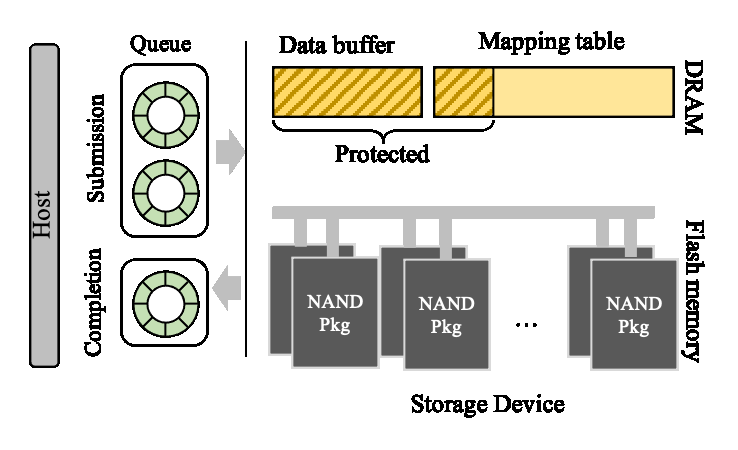
\includegraphics[width=0.4\textwidth]{figure/dawid_ssd_archi.eps}
    %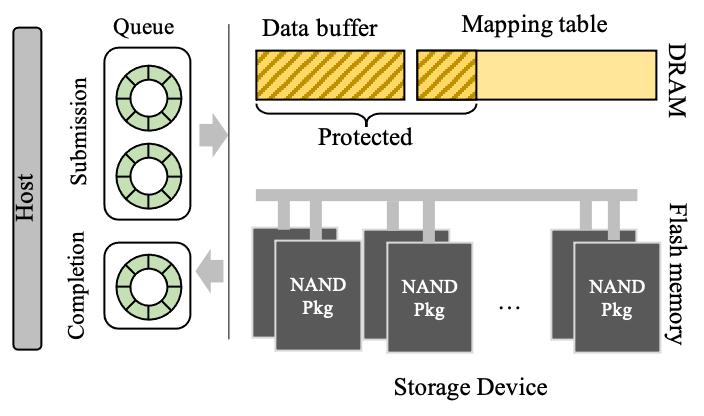
\includegraphics[width=0.4\textwidth]{figure/dawid_ssd_archi.png}
    \caption{\textbf{SSD architecture with \ours{} buffer.}}
    \label{fig_dawid_archi}
\end{figure}

This paper presents a device-internal buffer architecture called \ours{}
for the SSDs under capacitance constraints. 
% which operates under capacitance constraints.
Fig.~\ref{fig_dawid_archi} shows the SSD architecture targeted in our study. 
The data maintained in the buffer can be classified into two types: the actual user data and 
the metadata for SSD management (i.e, mapping table). 
When the buffer is partially protected, the number of dirty pages is limited to 
the maximum amount of data that the on-board capacitance can protect. 
If the number of dirty pages goes beyond the limit, changes should be flushed to the flash memory immediately
to meet the durability constraint for SSDs. 
% otherwise durability violated. 
% \EUNJI{
\ours{} applies this compromise only to the metadata, while protecting the user data entirely. 
The data write is not only synchronous with the user request, which hampers user experiences seriously when delayed, but also unrecoverable in the event of the power crash. 
\iffalse
because (1) the data write is synchronous with the user request and (2) the user data takes up a relatively 
small footprint in the buffer. 
\fi
% This is because the storage suffers from serious performance degradation when the user data 
% is not fully protected and should be entirely flushed upon a \texttt{FLUSH} command.
% }
% \textcolor{brown}{
% \ours{} essentially limits the number of dirty pages within buffer
% to the level the maximum capacitance can protect.
% If the number of dirty pages goes beyond the limit, changes are flushed to the flash memory. 
% }

\EUNJI{For this architecture, the problem boils down to how to reduce the write traffic to persist the mapping table to flash memory under capacitance constraints. 
% \iffalse
Reducing the synchronization overhead of the mapping table is a well-known problem and has been extensively studied for a past decade~\cite{jiang2011s, kim2017shrd}. 
However, they mostly focus on the SSDs without PLP, which have different properties to the PLP-SSDs with capacitance constraints. 
As opposed to the SSDs without capacitors, (1) the PLP-SSDs ensure data persistency immediately, and (2) there is no need to write-back the buffered data when protected. 
% \fi
In this regard, the \ours{} buffer aims at minimizing the \textit{dirty memory footprint} of the mapping table at any point in time. To this end, \ours{} processes outstanding requests in the order that least increases the number of dirty pages in the mapping table. 
This scheme not only reduces the number of flushes for the mapping table partially protected but also increases the efficiency of flush operation by aggregating more translation updates into the smaller translation pages.
}
% 그럼 이제 문제는 배터리 용량 제한으로 인해 발생하는 mapping table 의 추가적인 flash memory write 연산을 어떻게 효율적으로 다룰 것인가 하는 문제로 귀결된다. 
% 사실 mapping table 의 write-traffic 을 줄이는 연구는 well-known problem and has been studied extensively. 

% 우리가 제안하는 기법은 이 두 기법 사이에 있음. 보호가 가능한 분량 만큼에 대해서는 write-back 이 필요없으나, 해당 크기를 넘어서는 상황에서는 mapping table 의 효율적인 write-back 이 요구됨. 특히, 배터리가 전혀 없는  스토리지와 달리, 배터리로 보호되는 SSD는 버퍼에 쓰여진 데이터에 대해서도 모두 영속성을 보장하기 때문에 보호 가능한 범위를 벗어나는 순간 즉각적인 write-back 이 필요하다. 

% 이러한 상황을 고려했을 때, 버퍼 관리 기법에서 추구해야할 특성은 두가지로 생각해볼 수 있다. 

% 1) 매 순간 평균 dirty memory footprint 가 작아야 하고,  
% 2) 버퍼링 write-back cost 를 줄일 수 있도록 최대한 updates 를 aggregate 시킬 수 있어야 함. 

\EUNJI{The \ours{} buffer is built upon the current trend of increasing queue depth of the storage interfaces. SATA and SAS support a single queue with 32 and 245 commands, but NVMe has 
up to 65,535 queues with as many as 65,536 commands per queue. 
This extension allows SSDs to further optimize the internal activities by taking advantage of the outstanding request information.
By re-scheduling the requests in a way of reducing the write-back cost of the mapping table, the \ours{} buffer achieves high IOPS and low latency of SSDs at a small amount of capacitance. 
}
% https://blog.westerndigital.com/nvme-queues-explained/#:~:text=Both%20SATA%20and%20SAS%20interfaces,for%20capacity%20and%20performance%20scaling.

% 제안하는 기법은 상기 두 개의 목표를 달성하기 위해, 동일한 mapping table page 에 업데이트를 필요로하는 write 를 그룹핑하고, dirty memory footprint 의 증가를 가장 적게 일으키도록 write 
% 4GB인데 4KB 단위로 맵핑 테이블 유지하면, 1M 개의 entry. 4byte 면 4MB 임. 

% 우리는 이것을 device queue 의 depth 가 증가했다는 점을 이용하여 개선한다. 
% SSD의 병렬성을 최대한 활용하기 위해 queue 의 depth 는 증가함. NVMe 의 경우 최대 65535 의 queue를 지원하고 각각 65535 개의 outstanding commands 를 지원함. 
% 이것은 SSD 가 실행할 요청에 대한 정보를 가질 수 있도록 하여 SSD에 최적화 된 형태로 이를 활용할 수 있는 가능성을 준다. 
% Support for up to 65,535 I/O Queues, with each I/O Queue supporting up to 65,535 outstanding
% commands;
% 본 논문에서는 queue 에 있는 request 들을 re-ordering 하여 배터리 용량 제한 문제를 극복하기 위한 기법을 제안한다. 

\iffalse
Based on this underlying architecture, \ours{} performs an I/O scheduling 
for the write requests within storage queue to reduce the write traffic
caused by the capacitance limitation. The scheduling algorithm aims to minimize the dirty page footprint 
of the internal buffer at a given time window. This behavior can reduce the frequency at which the number of dirty pages
exceeds the threshold and the modified pages are forced to flash memory. 
To this end, \ours{} prioritizes the write request with the least increase 
of the number of dirty pages in the mapping table.
With this policy, the write request of which the associated mapping page is already dirty 
has a top priority because it does not add the dirty page count. For other cases,  
% When the mapping page in clean state should be updated, 
\ours{} groups the write requests that modify the same mapping page 
and process them in batch in the order of group size. 
This policy enhances buffering and coalescing of the changes to the mapping table in the buffer, 
reducing a flush overhead significantly under capacitance constraints
compared to the FIFO (First-In First-Out) scheduling policy currently used in SSDs. 
\fi

To evaluate the effectiveness of \ours, we implement the proposed buffer design
in \texttt{FEMU}, which is an open-source SSD development framework~\cite{li2018case}. The performance evaluation with various workloads 
shows that \ours{} reduces the write traffic by up to 78\% and provides 25\% higher IOPS 
compared to the FIFO scheduling scheme when only 10\% of the mapping table is protected. 
Compared to the full-protection architecture, \ours{} has has 20\% more writes and 
9\% of performance overhead, while reducing the required capacitance by 90\%. 

The remainder of this paper is organized as follows. In section 2, we briefly review the 
requirements and constraints for SSD with respect to reliability. Section 3 explains the 
design of SpartanSSD and Section 4 describes the implementation and performance evaluation results. 
Section 5 quantitatively analyzes the energy consumption of SSDs. Section 6 discusses our propoed design 
in relation to prior work, and Section 7 concludes. 


%define the cost for each data. the number of dirty pages increased 
% In contrast, the metadata is used only inside storage for device integrity or efficient indexing, 
% and thus it is more flexible to manage under capacitance constraints. 

%used for protecting device integrity and for accessing data 
% within storage. 

% In contrast, the metadata 
% user data 는 loss 가 발생하면 복구할 방법이 없는 반면, metadata 는 
% 사용자 데이터는 즉시 영구적으로 보호하는 것을 못한다면, 
% FLUSH command 처리에 따른 심각한 성능저하 초래. 
% host 는 반드시 flush command 를 보내야 하고, 그시점에 모든 데이터를 flush. 

% 반면 metadata 는 SSD가 해당 데이터를 잘 접근하고 SSD 자체의 integrity 유지를 위해 필요한 정보로, 
% 어느 정도 성능과 persistence 간의 

% protects user data 
%the storage buffer may be partially unprotected in power loss. 


\iffalse
\begin{itemize}
    \item capacitor density vs. SSD density 
    \item partially protected SSD 
    \item minimize the number of dirty page: write-back or management 
    \item user data cannot be managed by SSD 
    \item mapping table 의 더티 페이지 수를 줄일 수 있도록. 
\end{itemize}


A paragraph of text goes here.  Lots of text.  Plenty of interesting
text. \\

More fascinating text. Features\endnote{Remember to use endnotes, not footnotes!} galore, plethora of promises.\\
\fi
